% Options for packages loaded elsewhere
\PassOptionsToPackage{unicode}{hyperref}
\PassOptionsToPackage{hyphens}{url}
\PassOptionsToPackage{dvipsnames,svgnames,x11names}{xcolor}
%
\documentclass[
  letterpaper,
  DIV=11,
  numbers=noendperiod]{scrartcl}

\usepackage{amsmath,amssymb}
\usepackage{iftex}
\ifPDFTeX
  \usepackage[T1]{fontenc}
  \usepackage[utf8]{inputenc}
  \usepackage{textcomp} % provide euro and other symbols
\else % if luatex or xetex
  \usepackage{unicode-math}
  \defaultfontfeatures{Scale=MatchLowercase}
  \defaultfontfeatures[\rmfamily]{Ligatures=TeX,Scale=1}
\fi
\usepackage{lmodern}
\ifPDFTeX\else  
    % xetex/luatex font selection
\fi
% Use upquote if available, for straight quotes in verbatim environments
\IfFileExists{upquote.sty}{\usepackage{upquote}}{}
\IfFileExists{microtype.sty}{% use microtype if available
  \usepackage[]{microtype}
  \UseMicrotypeSet[protrusion]{basicmath} % disable protrusion for tt fonts
}{}
\makeatletter
\@ifundefined{KOMAClassName}{% if non-KOMA class
  \IfFileExists{parskip.sty}{%
    \usepackage{parskip}
  }{% else
    \setlength{\parindent}{0pt}
    \setlength{\parskip}{6pt plus 2pt minus 1pt}}
}{% if KOMA class
  \KOMAoptions{parskip=half}}
\makeatother
\usepackage{xcolor}
\setlength{\emergencystretch}{3em} % prevent overfull lines
\setcounter{secnumdepth}{-\maxdimen} % remove section numbering
% Make \paragraph and \subparagraph free-standing
\makeatletter
\ifx\paragraph\undefined\else
  \let\oldparagraph\paragraph
  \renewcommand{\paragraph}{
    \@ifstar
      \xxxParagraphStar
      \xxxParagraphNoStar
  }
  \newcommand{\xxxParagraphStar}[1]{\oldparagraph*{#1}\mbox{}}
  \newcommand{\xxxParagraphNoStar}[1]{\oldparagraph{#1}\mbox{}}
\fi
\ifx\subparagraph\undefined\else
  \let\oldsubparagraph\subparagraph
  \renewcommand{\subparagraph}{
    \@ifstar
      \xxxSubParagraphStar
      \xxxSubParagraphNoStar
  }
  \newcommand{\xxxSubParagraphStar}[1]{\oldsubparagraph*{#1}\mbox{}}
  \newcommand{\xxxSubParagraphNoStar}[1]{\oldsubparagraph{#1}\mbox{}}
\fi
\makeatother


\providecommand{\tightlist}{%
  \setlength{\itemsep}{0pt}\setlength{\parskip}{0pt}}\usepackage{longtable,booktabs,array}
\usepackage{calc} % for calculating minipage widths
% Correct order of tables after \paragraph or \subparagraph
\usepackage{etoolbox}
\makeatletter
\patchcmd\longtable{\par}{\if@noskipsec\mbox{}\fi\par}{}{}
\makeatother
% Allow footnotes in longtable head/foot
\IfFileExists{footnotehyper.sty}{\usepackage{footnotehyper}}{\usepackage{footnote}}
\makesavenoteenv{longtable}
\usepackage{graphicx}
\makeatletter
\def\maxwidth{\ifdim\Gin@nat@width>\linewidth\linewidth\else\Gin@nat@width\fi}
\def\maxheight{\ifdim\Gin@nat@height>\textheight\textheight\else\Gin@nat@height\fi}
\makeatother
% Scale images if necessary, so that they will not overflow the page
% margins by default, and it is still possible to overwrite the defaults
% using explicit options in \includegraphics[width, height, ...]{}
\setkeys{Gin}{width=\maxwidth,height=\maxheight,keepaspectratio}
% Set default figure placement to htbp
\makeatletter
\def\fps@figure{htbp}
\makeatother

\KOMAoption{captions}{tableheading}
\makeatletter
\@ifpackageloaded{caption}{}{\usepackage{caption}}
\AtBeginDocument{%
\ifdefined\contentsname
  \renewcommand*\contentsname{Table of contents}
\else
  \newcommand\contentsname{Table of contents}
\fi
\ifdefined\listfigurename
  \renewcommand*\listfigurename{List of Figures}
\else
  \newcommand\listfigurename{List of Figures}
\fi
\ifdefined\listtablename
  \renewcommand*\listtablename{List of Tables}
\else
  \newcommand\listtablename{List of Tables}
\fi
\ifdefined\figurename
  \renewcommand*\figurename{Figure}
\else
  \newcommand\figurename{Figure}
\fi
\ifdefined\tablename
  \renewcommand*\tablename{Table}
\else
  \newcommand\tablename{Table}
\fi
}
\@ifpackageloaded{float}{}{\usepackage{float}}
\floatstyle{ruled}
\@ifundefined{c@chapter}{\newfloat{codelisting}{h}{lop}}{\newfloat{codelisting}{h}{lop}[chapter]}
\floatname{codelisting}{Listing}
\newcommand*\listoflistings{\listof{codelisting}{List of Listings}}
\makeatother
\makeatletter
\makeatother
\makeatletter
\@ifpackageloaded{caption}{}{\usepackage{caption}}
\@ifpackageloaded{subcaption}{}{\usepackage{subcaption}}
\makeatother

\ifLuaTeX
  \usepackage{selnolig}  % disable illegal ligatures
\fi
\usepackage{bookmark}

\IfFileExists{xurl.sty}{\usepackage{xurl}}{} % add URL line breaks if available
\urlstyle{same} % disable monospaced font for URLs
\hypersetup{
  pdftitle={Formation médiation numérique},
  pdfauthor={Anne-Laure Donzel},
  colorlinks=true,
  linkcolor={blue},
  filecolor={Maroon},
  citecolor={Blue},
  urlcolor={Blue},
  pdfcreator={LaTeX via pandoc}}


\title{Formation médiation numérique}
\usepackage{etoolbox}
\makeatletter
\providecommand{\subtitle}[1]{% add subtitle to \maketitle
  \apptocmd{\@title}{\par {\large #1 \par}}{}{}
}
\makeatother
\subtitle{AAF - novembre 2024}
\author{Anne-Laure Donzel}
\date{}

\begin{document}
\maketitle


\section{Présentation de la
formation}\label{pruxe9sentation-de-la-formation}

\subsection{Objectifs de la formation}\label{objectifs-de-la-formation}

\begin{itemize}
\tightlist
\item
  S'interroger sur les pratiques
\item
  Découvrir des outils
\item
  Partager des exemples
\end{itemize}

\subsection{Limites de la formation}\label{limites-de-la-formation}

\begin{itemize}
\tightlist
\item
  Sélection d'outils forcément partiale
\item
  Peu de temps pour manipuler
\item
  La seule limite = créativité
\end{itemize}

\subsection{Déroulé}\label{duxe9rouluxe9}

\begin{itemize}
\item
  \textbf{Jeudi 21 novembre}
\item
  Introduction
\item
  Outillage : créer des avant/après
\item
  Outillage : créer des frises chronologiques
\item
  Méthodologie : préparer ses fichiers
\end{itemize}

\begin{itemize}
\item
  \textbf{Vendredi 22 novembre}
\item
  Méthodologie : préparer ses fichiers - suite
\item
  Outillage : créer des cartes
\item
  Outillage : créer des cartes narratives
\item
  Conclusion
\end{itemize}

\section{Quelles sont les pratiques de médiation dans vos services
?}\label{quelles-sont-les-pratiques-de-muxe9diation-dans-vos-services}

\section{Introduction}\label{introduction}

\subsection{Médiation-facilitation et
médiation-valorisation}\label{muxe9diation-facilitation-et-muxe9diation-valorisation}

\includegraphics{img/arch_paris_med_facilitation.png} Légende :
\href{https://archives.paris.fr/_depot_ad75/_depot_arko/articles/2622/fiche-d-aide-a-la-recherche-jugement-civil_doc.pdf}{\emph{outil
d'aide à la recherche des Archives de Paris}}

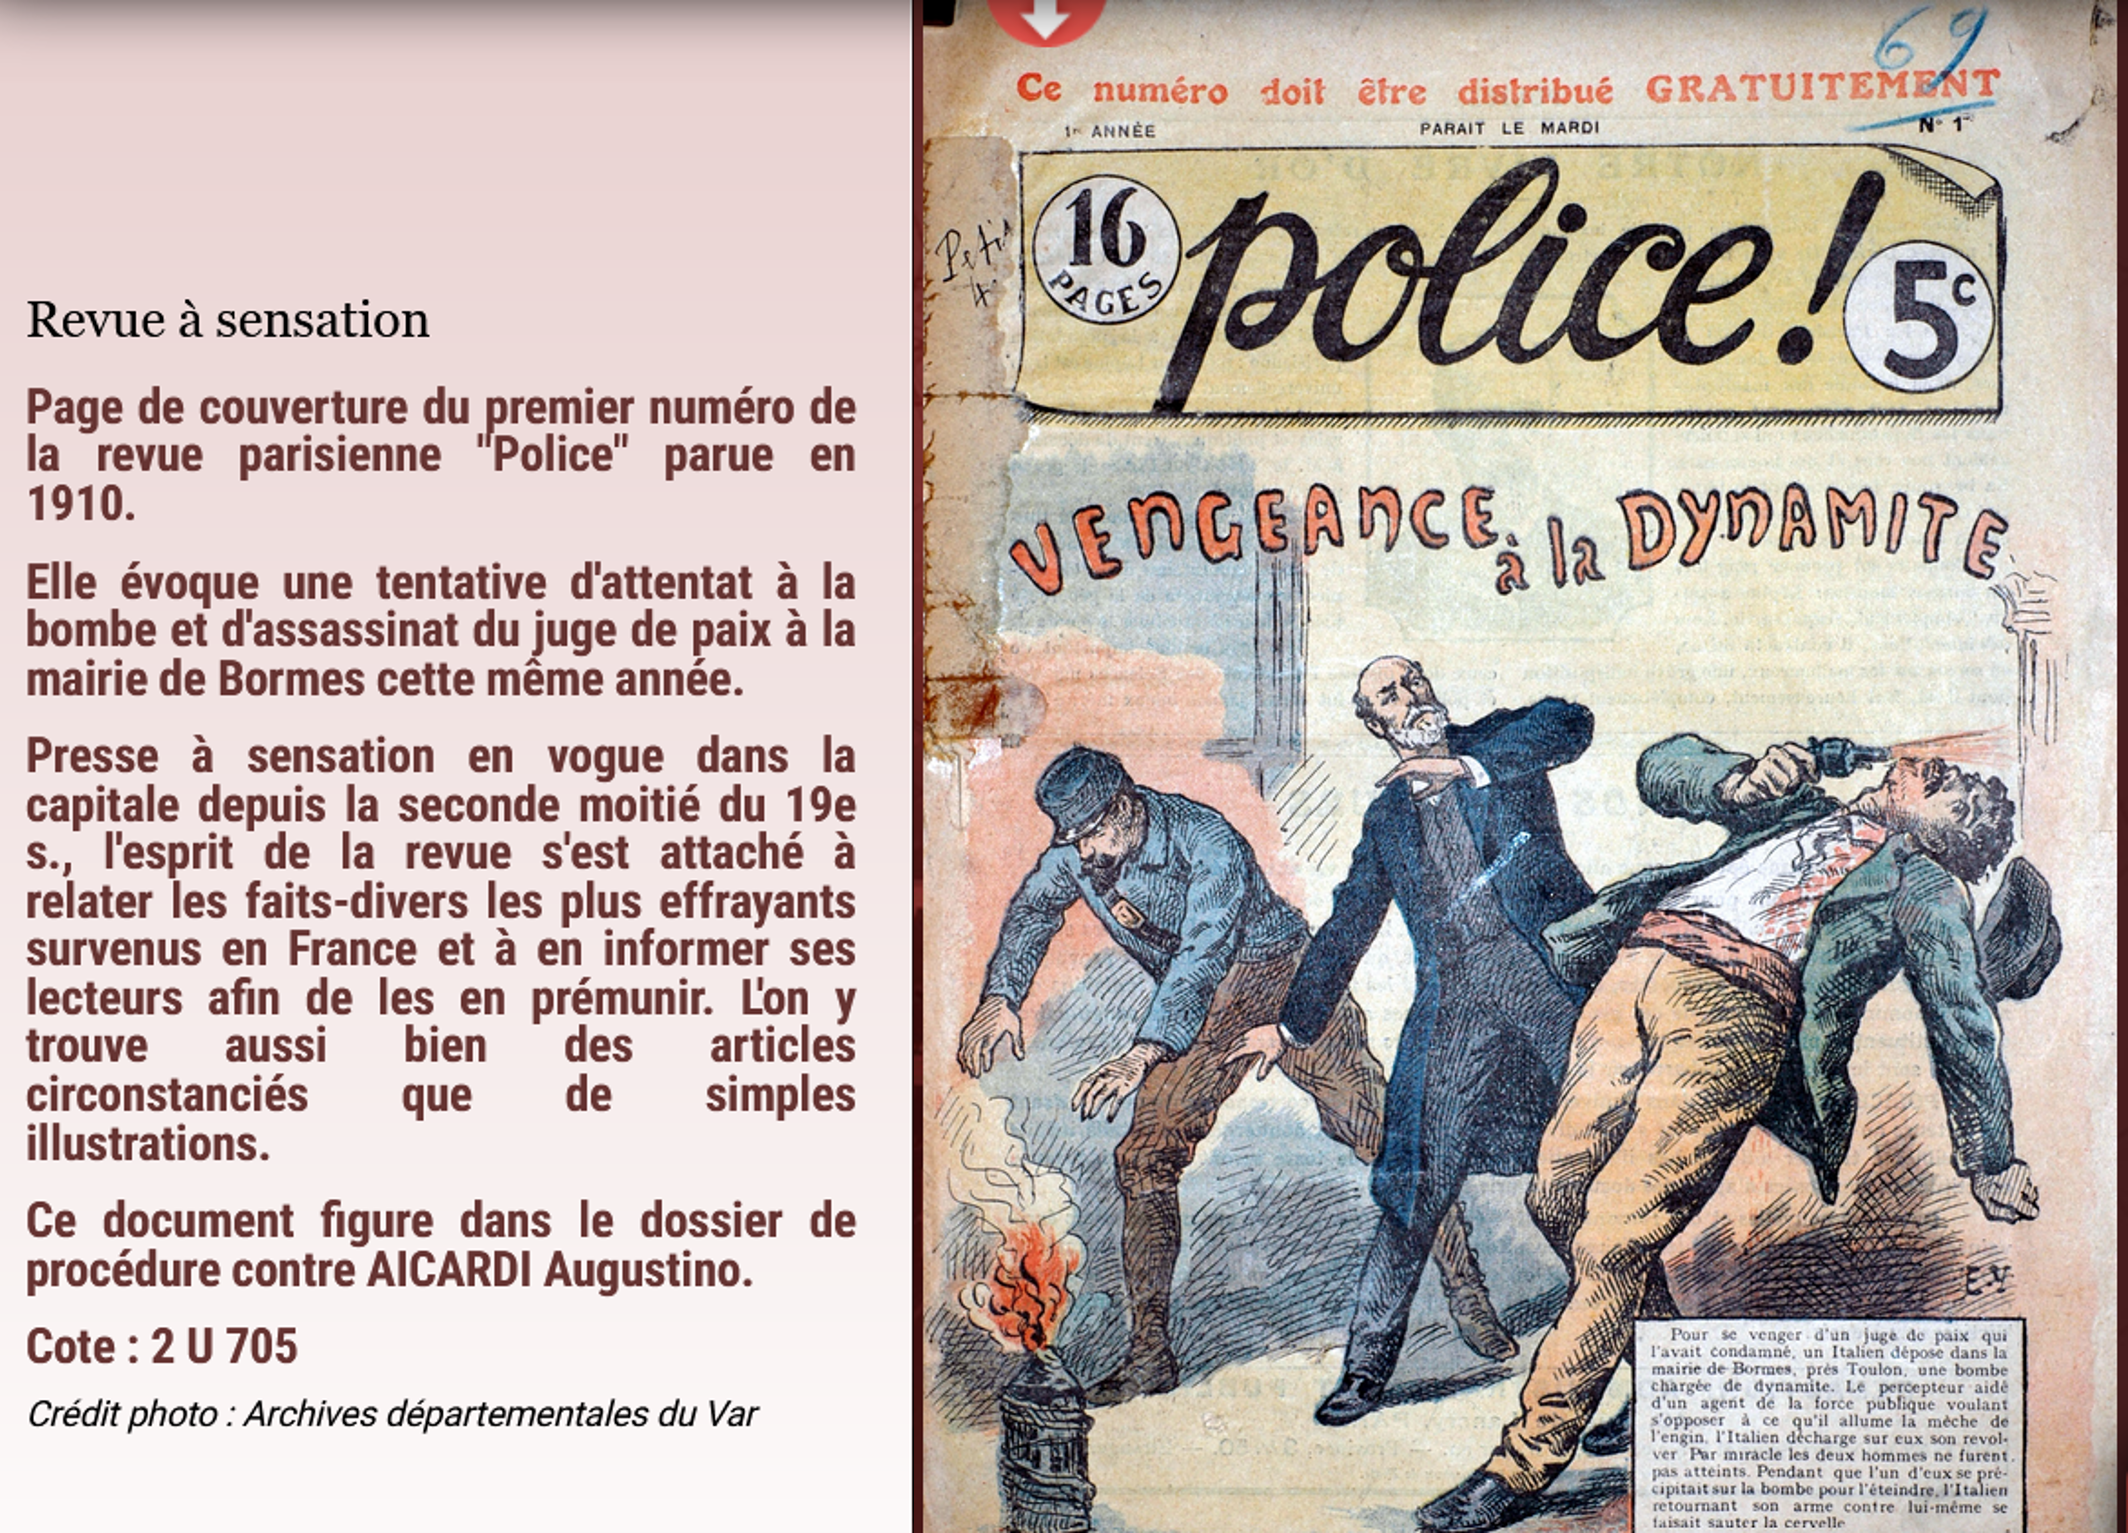
\includegraphics{img/arch_var_med_valo.png} Légende : extrait de
l'exposition virtuelle des AD83
\href{https://archives.var.fr/article.php?larub=308&titre=que-justice-soit-faite-methodes-d-investigations-varoises-1811-1958-}{\emph{Que
justice sois faite ! Méthodes d'investigations varoises (1811-1958)}}

traditionnellement : 2 types de médiation. D'un côté celle qui guide le
lecteur dans les fonds et de l'autre celle qui suscite l'intérêt du
public.

\subsection{De la médiation à la médiation
numérique}\label{de-la-muxe9diation-uxe0-la-muxe9diation-numuxe9rique}

\begin{itemize}
\tightlist
\item
  Faire comprendre et faciliter la capacité à s'emparer d'un sujet
\item
  Diffuser autrement
\item
  Toucher d'autres publics
\item
  Exploiter de nouveaux formats
\end{itemize}

Comment définir la médiation numérique ?

\begin{itemize}
\tightlist
\item
  Utilise les potentialités du numérique
\item
  Multimédia ou ``cross-média''
\item
  Ne se limite pas aux réseaux sociaux
\end{itemize}

la diffusion des archives en ligne pose la question d'une autre forme de
médiation. Cette diffusion remet partiellement en cause le rapport
traditionnel entre « sachant » et « non sachant » ; partiellement, car
les documents sont théoriquement accessibles et utilisables par tous.
Mais sans grille de lecture pour décoder, le sont-ils vraiment ?

\subsection{La médiation pour : accéder aux
fonds}\label{la-muxe9diation-pour-accuxe9der-aux-fonds}

La médiation numérique peut servir à présenter les données de gestion du
service, notamment pour faciliter l'accès aux fonds.

Exemple :
\href{https://archives.lillemetropole.fr/n/navigation-dans-les-fonds/n:512}{Naviguez
dans les fonds de la MEL}

\begin{center}
\includegraphics[width=0.3\textwidth,height=\textheight]{img/mel_fonds.png}
\end{center}

\subsection{La médiation pour : contextualiser les
fonds}\label{la-muxe9diation-pour-contextualiser-les-fonds}

Les outils numériques peuvent aussi permettre de réaliser des éléments
d'accompagnement à la recherche : présentation d'éléments historiques
locaux.

Exemple :
\href{https://archives.orleans-metropole.fr/histoires-dorleans/lencyclo}{L'Encycl'O
des archives municipales d'Orléans}

\begin{center}
\includegraphics{img/encyclo.png}
\end{center}

\subsection{La médiation pour : valoriser un fonds ou un
sujet}\label{la-muxe9diation-pour-valoriser-un-fonds-ou-un-sujet}

Les 2 objectifs précédents sont assez nouveaux avec le numérique, en
revanche, la valorisation des fonds grâce aux outils numériques se
situent dans la droite ligne de ce que les services pouvaient déjà
faire, mais avec un petit truc en plus.

Exemple :
\href{https://archives.valdemarne.fr/patrimoine-et-histoire/autour-de-nos-expositions/les-val-de-marnais-le-climat-et-lenvironnement}{Exposition
+ 2°C ? Les Val-de-Marnais, le climat et l'environnement}, qui propose
une expérience assez complète de médiation.

\begin{center}
\includegraphics{img/expo94.jpg}
\end{center}

\subsection{Autres exemples}\label{autres-exemples}

\href{https://www.pinterest.fr/archivesmanche/archives-gif/}{\textbf{Les
GIF des AD50}}

\textbf{Les puzzles :}

\begin{itemize}
\item
  \href{https://archives.lillemetropole.fr/jeux/puzzles/n:57}{Archives
  de la MEL}
\item
  \href{https://archives.hautesavoie.fr/jeux/puzzles/n:57}{AD de
  Haute-Savoie}
\end{itemize}

\textbf{Les associations de paires :}

\begin{itemize}
\item
  \href{https://archives.aisne.fr/jeux/jeux-de-paire/n:65}{AD de
  l'Aisne}
\item
  \href{https://archives.ville-saint-denis.fr/jeux/jeux-de-paire/n:11}{AM
  de Saint-Denis}
\end{itemize}

\textbf{Les quizz :}

\begin{itemize}
\item
  \href{https://www.archivesdepartementales76.net/quizz/quizzbyid/n:182}{AD
  de Seine-Maritime}
\item
  \href{https://www.archives13.fr/n/quiz-aco/n:239}{AD des
  Bouches-du-Rhône}
\end{itemize}

\section{A votre avis : quelles sont les indispensables pour lancer un
projet
?}\label{a-votre-avis-quelles-sont-les-indispensables-pour-lancer-un-projet}

\section{Les indispensables pour se
lancer}\label{les-indispensables-pour-se-lancer}

\subsection{Une stratégie}\label{une-stratuxe9gie}

Qu'allez-vous chercher à faire ? Quelle sera l'ojectif de vos actions de
médiation ? Est-ce que cela s'inscrit dans un projet de service ?

\begin{center}
\includegraphics{img/felix-mittermeier-nAjil1z3eLk-unsplash.jpg}
\end{center}

\subsection{Une réflexion
cohérente}\label{une-ruxe9flexion-cohuxe9rente}

Parfois, les actions de médiation se perdent dans les sites des services
et elles sont peu mises en avant. Si votre service y consacre du temps,
il faut que cela soit visible.

\begin{center}
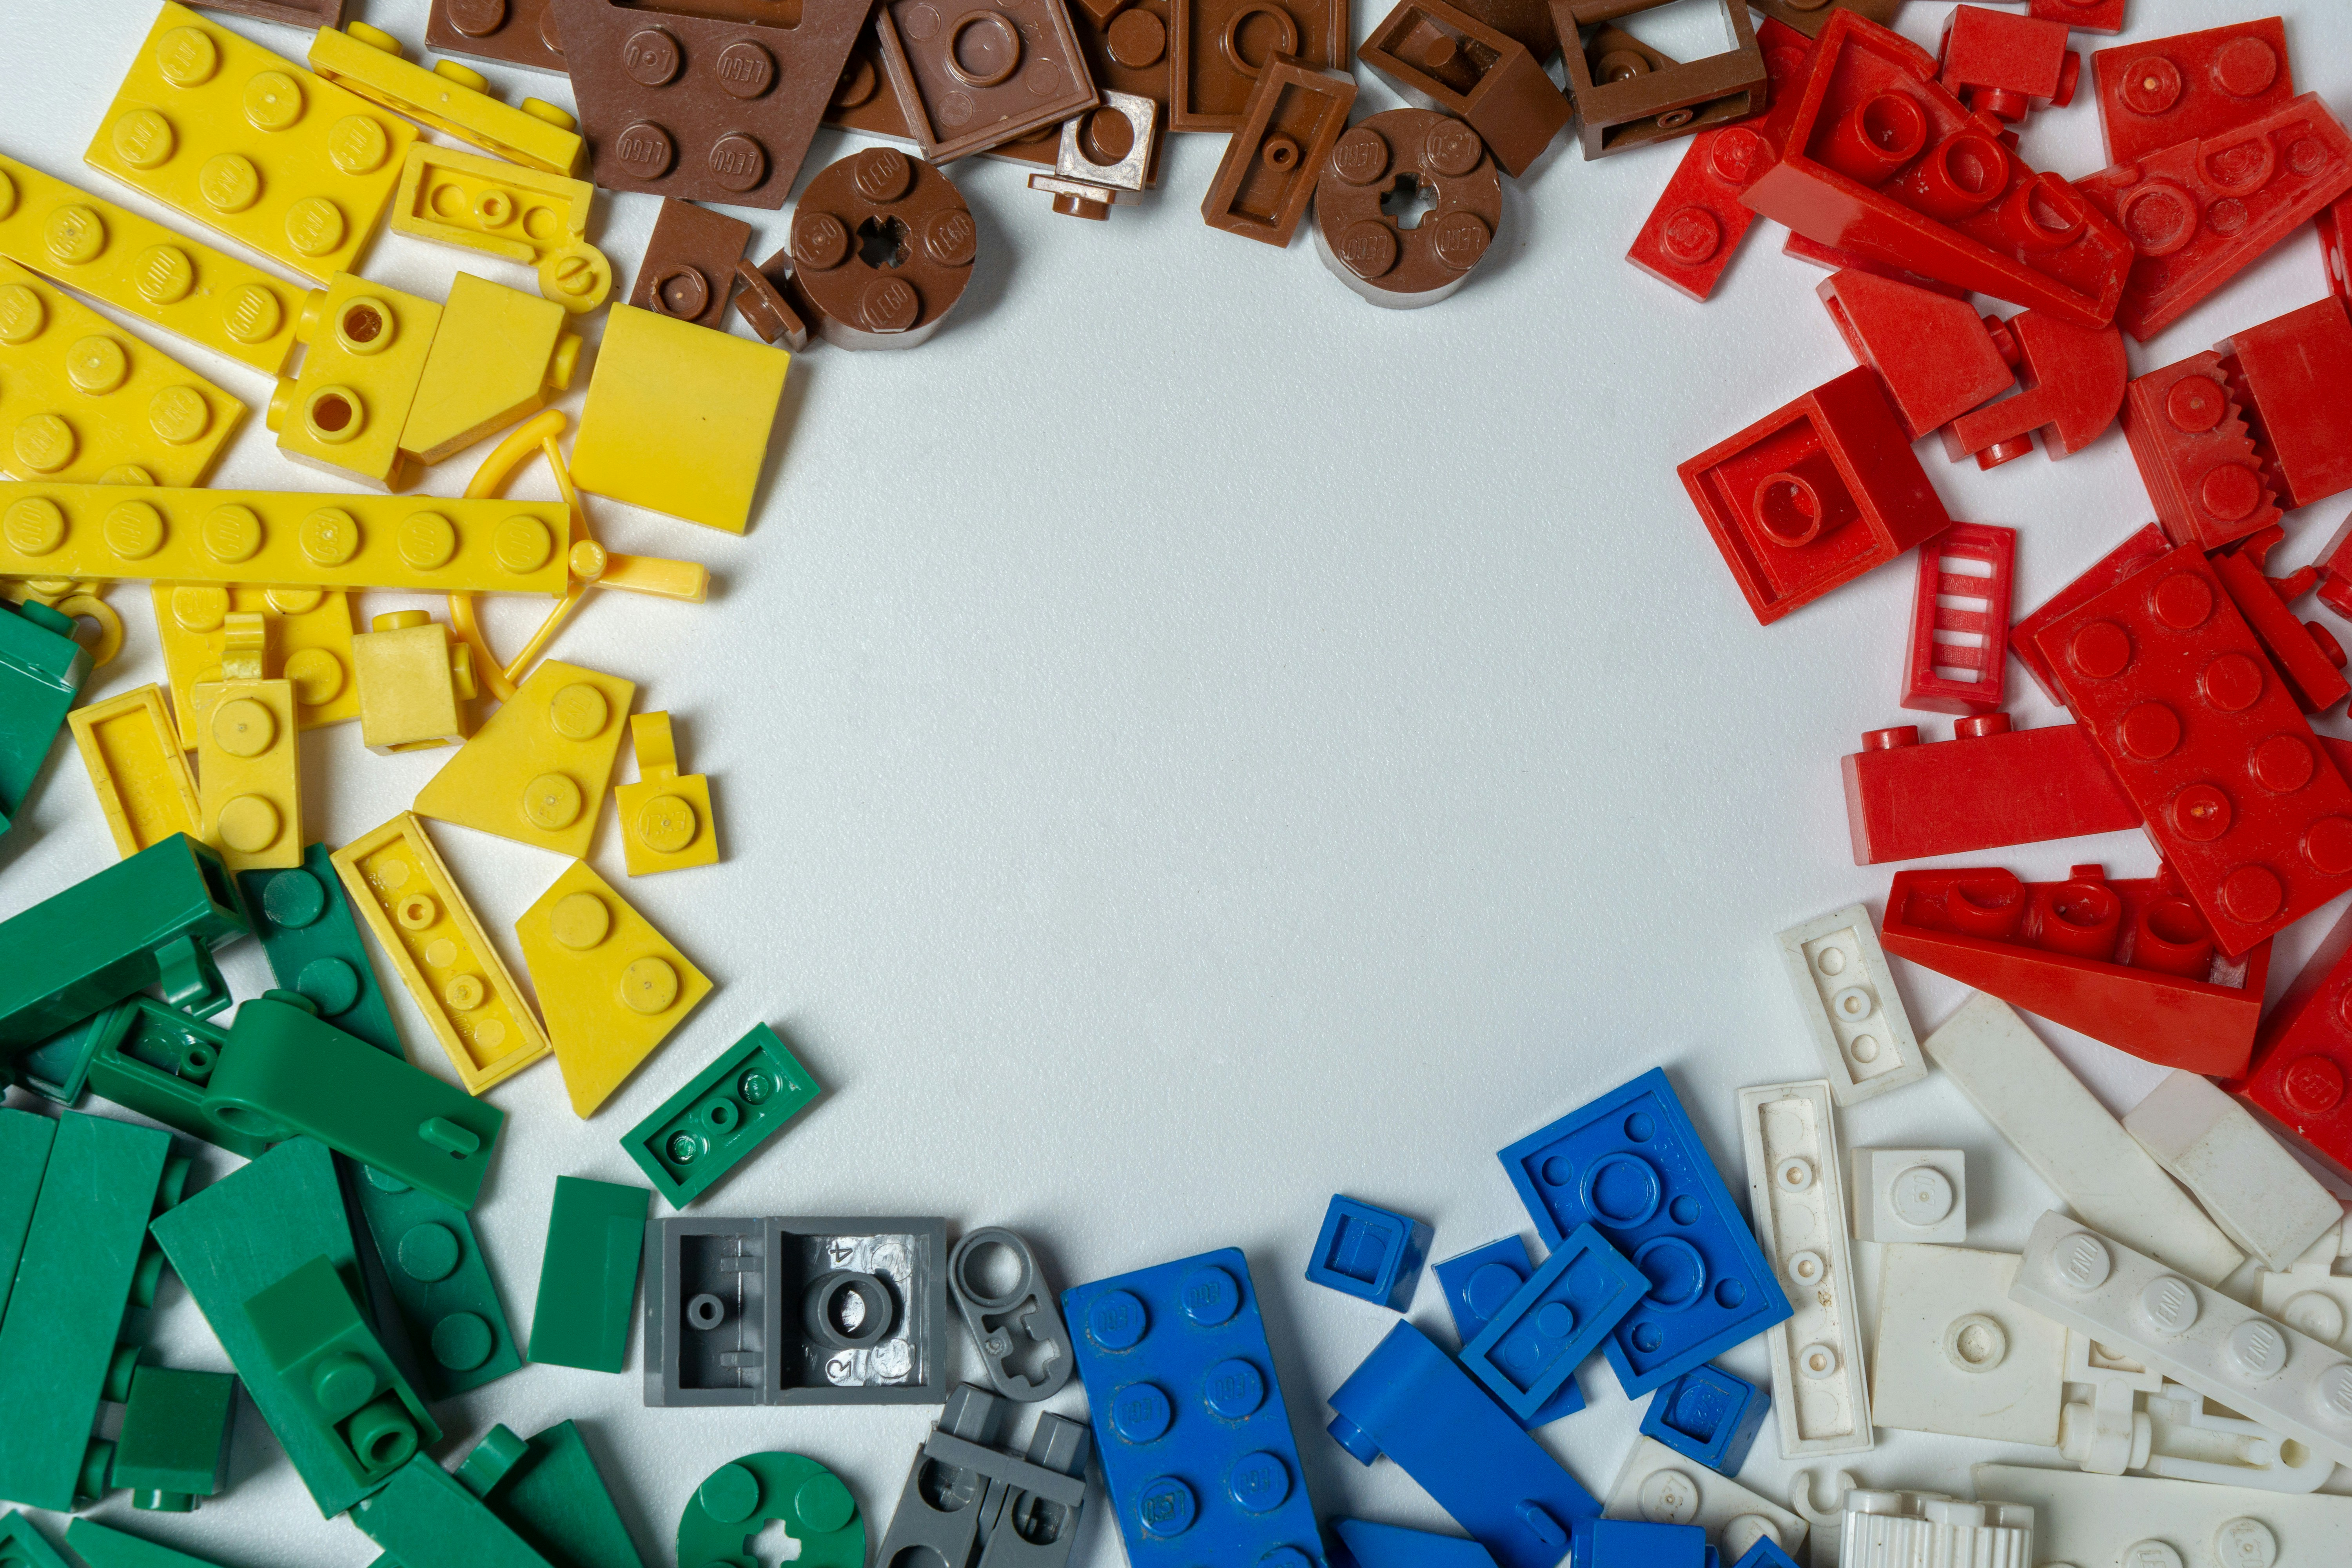
\includegraphics{img/mourizal-zativa-gNMVpAPe3PE-unsplash.jpg}
\end{center}

\subsection{Des publics}\label{des-publics}

Les publics des archives sont nombreux et variés : chercheurs
(expérimentés ou non), généalogistes, enfants lors d'action pédagogique,
curieux\ldots{} \begin{center}
\includegraphics{img/patrick-federi-RshUMrKap-0-unsplash.jpg}
\end{center}

\subsection{Des compétences}\label{des-compuxe9tences}

C'est au coeur de cette formation ! derrières les actions de médiation,
il y a des agents : qui s'en charge ? avec quels moyens ? quel
accompagnement ?

\begin{center}
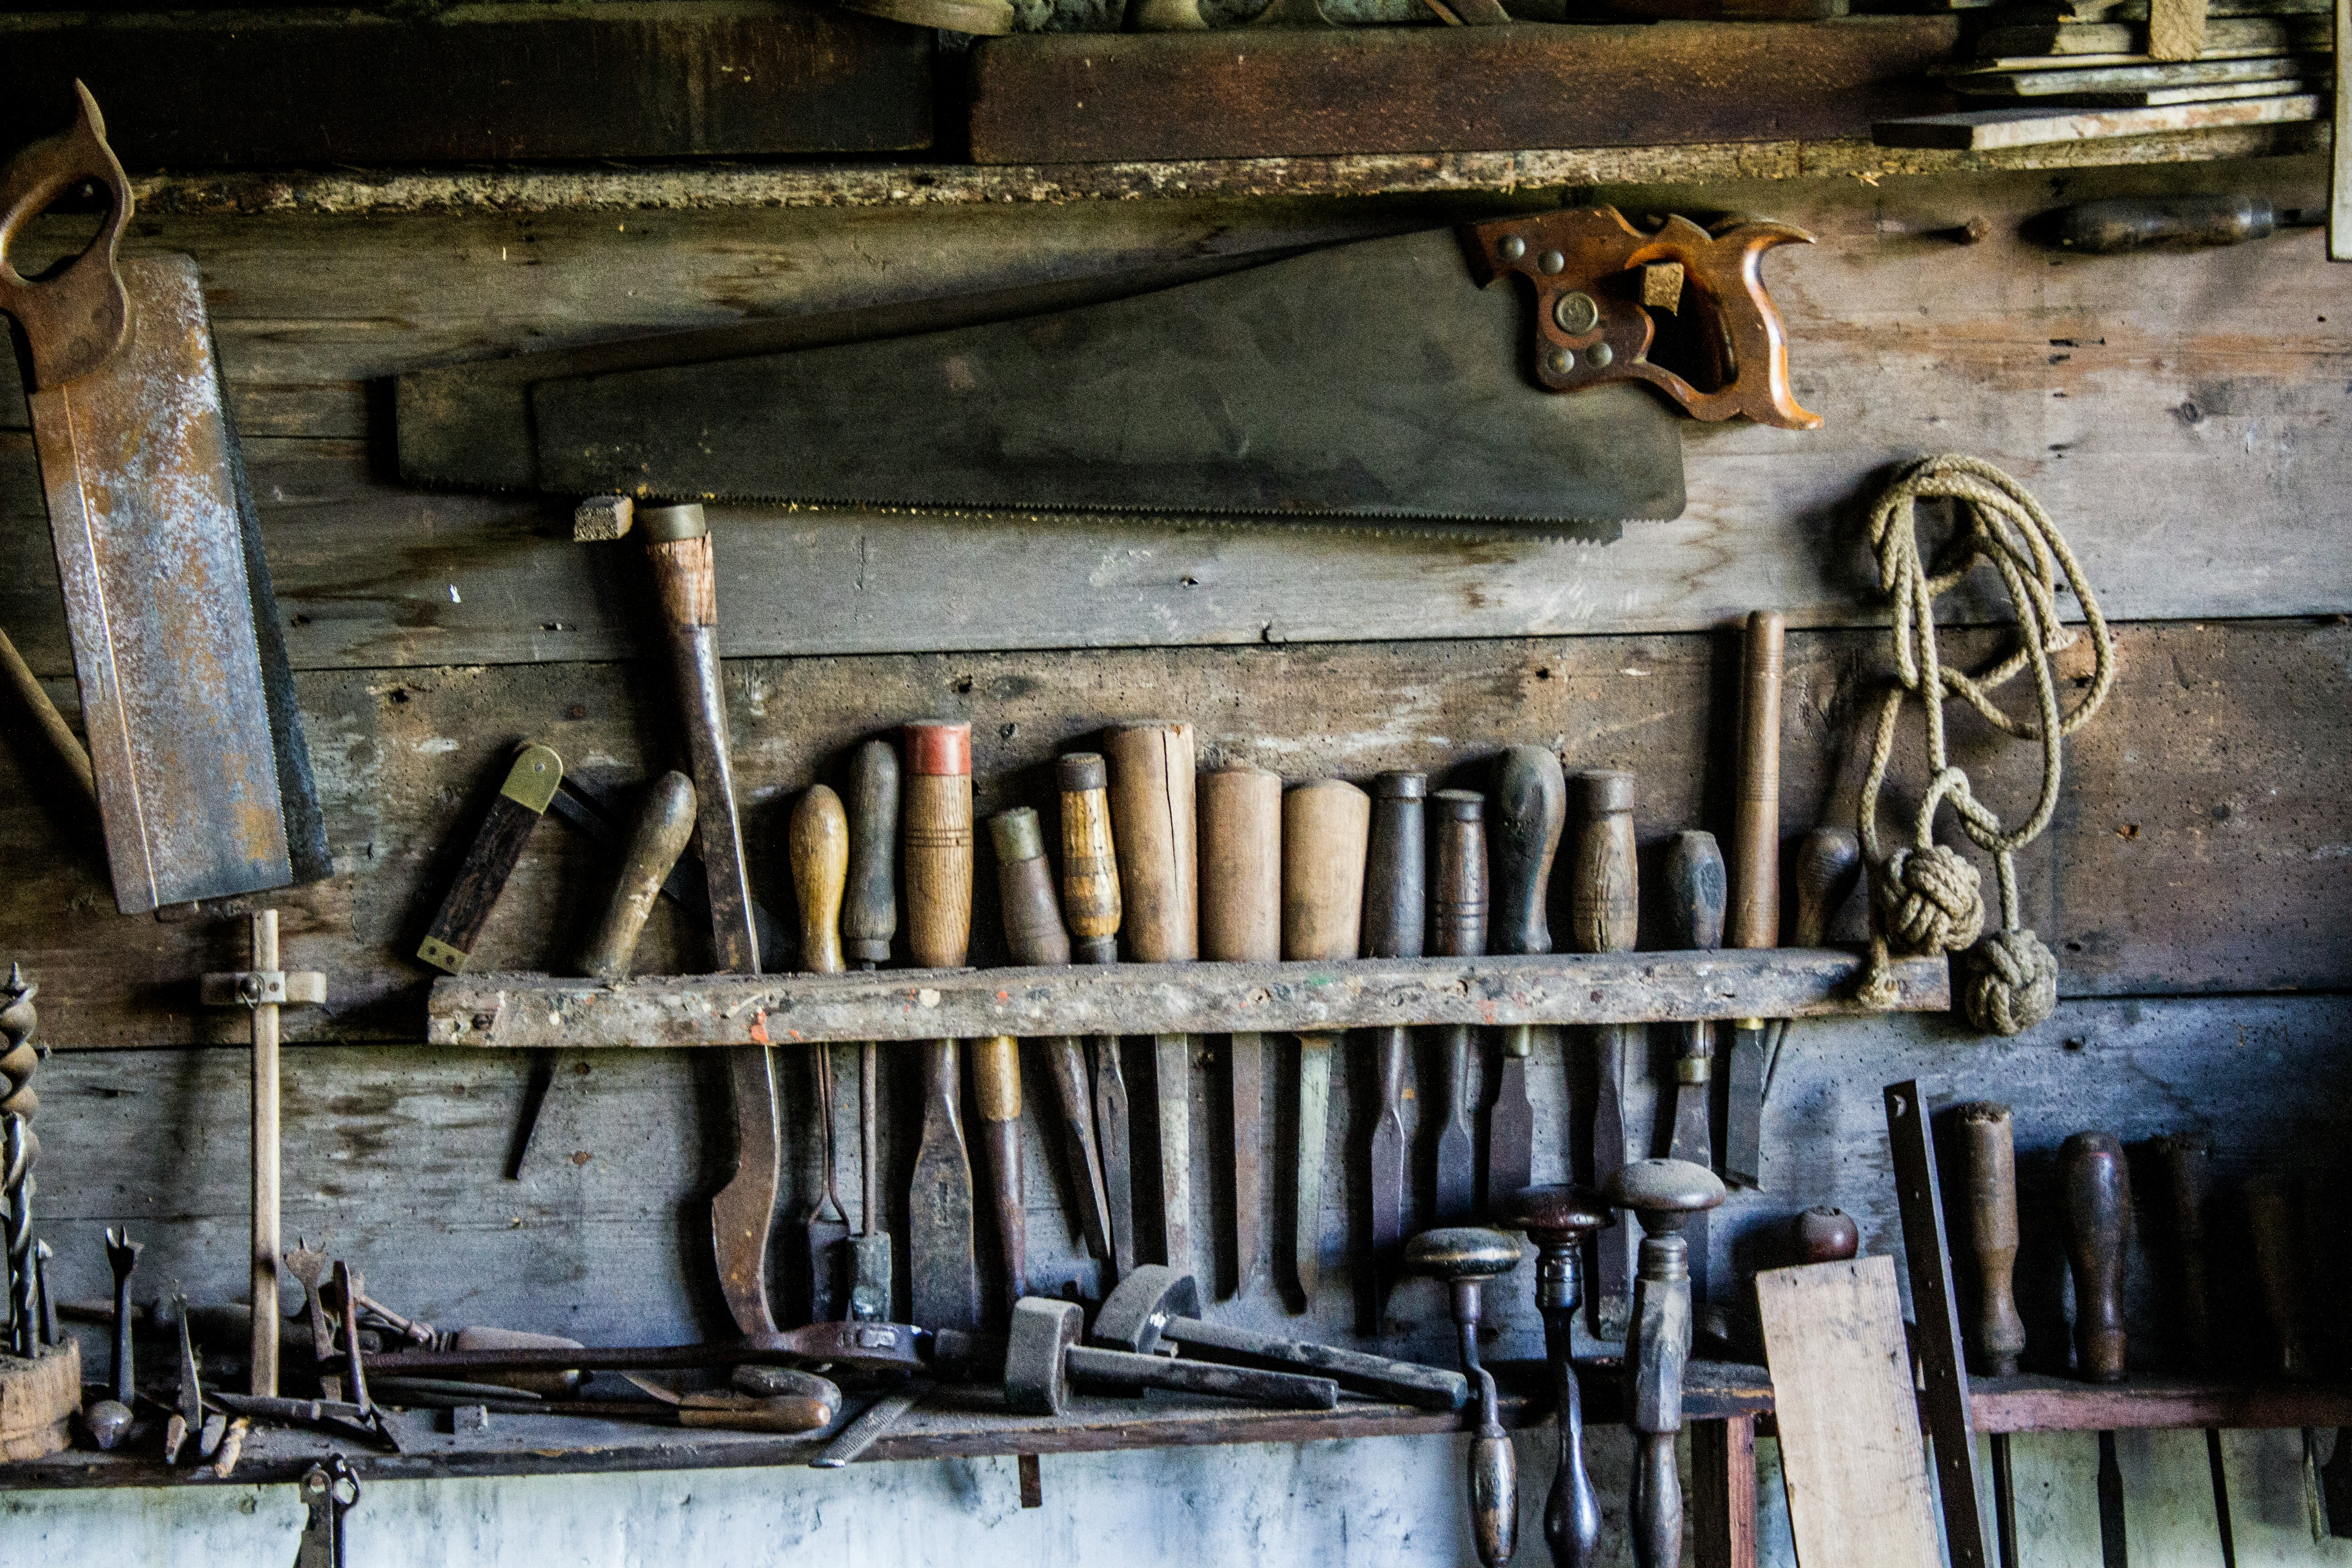
\includegraphics{img/philip-swinburn-vS7LVkPyXJU-unsplash.jpg}
\end{center}

\subsection{Des données}\label{des-donnuxe9es}

Peu importe ce que vous allez chercher à faire : il va vous falloir des
données ! et, assez vite, vous allez voir qu'elles ont souvent plein de
petits défauts.

\begin{quote}
De quelles données disposez-vous dans vos services ?
\end{quote}

\begin{center}
\includegraphics{img/google-deepmind-Oy2yXvl1WLg-unsplash.jpg}
\end{center}

\section{Les types de format}\label{les-types-de-format}

\begin{center}
\includegraphics{img/categ-formats.gif}
\end{center}

\section{Nos tests d'outils}\label{nos-tests-doutils}

\subsection{Qu'allons nous faire ?}\label{quallons-nous-faire}

\begin{itemize}
\item
  Créer des avant/après à partir de photos
\item
  Créer des frises chronologiques
\item
  Créer des cartes
\item
  Créer des graphiques
\item
  Créer des dispositifs multimédias
\end{itemize}

Et nous apprendrons aussi à nettoyer et enrichir des données

Pour chaque outil, nous aurons des exercices simples et des plus
complexes, et vous repartirez avec tous les tuto et pas à pas des
exercices simples.

\section{Créer des avant/après à partir de
photos}\label{cruxe9er-des-avantapruxe8s-uxe0-partir-de-photos}

\subsection{Pourquoi faire ?}\label{pourquoi-faire}

\begin{itemize}
\item
  Mettre en avant les transformations d'un territoire ou d'un lieu

  \begin{itemize}
  \tightlist
  \item
    \href{https://archives.aubervilliers.fr/De-la-salle-des-fetes-au-Theatre-de-la-Commune}{Evolution
    du Théâtre de la Commune, Aubervilliers}
  \end{itemize}
\item
  Valoriser le travail du service des archives

  \begin{itemize}
  \item
    \href{https://www.archives13.fr/n/l-education-des-vers-a-soie/n:242}{Montrer
    le travail de restauration}
  \item
    \href{https://www.archives-loiret.fr/nouveau-batiment/les-archives-demenagent/en-attendant-le-demenagement}{Communiquer
    sur le conditionnement}
  \end{itemize}
\end{itemize}

\subsection{Comment faire ?}\label{comment-faire}

Nous allons utiliser l'outil :
\href{https://juxtapose.knightlab.com/}{JuxtaposeJS}

\begin{center}
\includegraphics{img/juxtapose-gif.gif}
\end{center}

\section{Créer des frises
chronologiques}\label{cruxe9er-des-frises-chronologiques}

\subsection{Pourquoi faire ?}\label{pourquoi-faire-1}

\begin{itemize}
\item
  Positionner des évènements dans le temps

  \begin{itemize}
  \item
    Une histoire du territoire :
    \href{https://patrimoine.landerneau.bzh/chronologie/histoire-de-landerneau-10/n:64}{Archives
    municipales de Landerneau}
  \item
    Une histoire au jour le jour :
    \href{https://archives.aisne.fr/chronologies/n:134}{Archives
    départementales de l'Aisne}
  \end{itemize}
\end{itemize}

\subsection{Comment faire ?}\label{comment-faire-1}

Nous allons utiliser l'outil :
\href{https://timeline.knightlab.com/}{TimelineJS}

\begin{enumerate}
\def\labelenumi{\arabic{enumi}.}
\item
  Exercice 1 :
  \href{https://cdn.knightlab.com/libs/timeline3/latest/embed/index.html?source=14iK4j7BjoIyALvg4GhgJpOQD9MlAo0iAp72Byl_LYJc&font=Default&lang=en&initial_zoom=2&height=650}{frise
  chronologique des députés}
\item
  Exercice 2 : frise de l'AAF
\end{enumerate}

\subsection{Quelques bonnes pratiques}\label{quelques-bonnes-pratiques}

\begin{itemize}
\item
  Illustrer chaque évènement
\item
  Eviter les chronologie trop longue (ou bien penser votre navigation)
\item
  Ne penser pas la chronologie aussi comme un outil pour raconter des
  petites histoires. cela fonctionne très bien avec 20 évènements se
  déroulant sur 15 jours.
\end{itemize}

\section{Créer des cartes}\label{cruxe9er-des-cartes}

\subsection{Pourquoi faire ?}\label{pourquoi-faire-2}

\begin{itemize}
\item
  Localiser des fonds et offrir aux usagers une autre façon d'entrer
  dans les collections :
  \href{https://umap.openstreetmap.fr/fr/map/communes-du-calvados_1088012\#10/49.1220/-0.3543}{AD
  du Calvados} ou
  \href{https://patrimoines-archives.morbihan.fr/naviguer-par-carte}{AD
  du Morbihan}
\item
  Très adapté aux
  \href{https://umap.openstreetmap.fr/fr/map/carte-des-photos-en-open-data-des-am-de-marseille_628303\#12/43.3266/5.4252}{fonds
  iconographiques}
\item
  Très apprécié pour la
  \href{(https://umap.openstreetmap.fr/fr/map/documents-figures-des-archives-departementales-des_150869\#8/48.146/-1.950)}{réutilisation}
\item
  Rendre
  \href{https://archives.orleans-metropole.fr/sources-et-ressources-en-ligne/instruments-de-recherche/autorisations-durbanisme/visualisation-dynamique-des-permis-de-construire-de-1945-a-2007}{visible
  des phénomènes}
\end{itemize}

\subsection{Comment faire ?}\label{comment-faire-2}

Nous allons utiliser l'outil :
\href{https://umap.openstreetmap.fr/fr/}{uMap}

\section{Nettoyer et enrichir des
données}\label{nettoyer-et-enrichir-des-donnuxe9es}

\subsection{Comment avoir les ``bonnes données''
?}\label{comment-avoir-les-bonnes-donnuxe9es}

Pour les exercices de cartes ou de frises chronologiques : nous avons un
peu triché car les données étaient toutes prêtes.

Mais le plus souvent, on part d'un fichier où il manque des informations
et qui est mal structuré.

\begin{center}
\includegraphics{img/jeshoots-com-__ZMnefoI3k-unsplash.jpg}
\end{center}

\subsection{Comment faire ?}\label{comment-faire-3}

L'outil pour tout faire : \textbf{Open Refine}

\includegraphics{img/logooperefine.png}

\section{Créer des cartes
narratives}\label{cruxe9er-des-cartes-narratives}

\subsection{Pourquoi faire ?}\label{pourquoi-faire-3}

Les cartes type uMap sont parfois un peu figées et on aimerait les
enrichir de différents médias. Elles permettent aussi de réunir tout ce
qu'on a vu précédemment.

\begin{itemize}
\item
  Exemple des
  \href{https://storymaps.arcgis.com/collections/9a11ba9ba4fa40389c188924aad51844?item=1}{Archives
  de Poitiers}
\item
  Exemple des
  \href{https://storymaps.arcgis.com/stories/e2cefbbcdb7d498289241459af733416}{Archives
  d'Orléans}
\item
  Exemple des
  \href{https://www.archives13.fr/n/l-exposition-coloniale-de-marseille-de/n:298}{Archives
  départementales des Bouches-du-Rhône}
\end{itemize}

\subsection{Comment faire ?}\label{comment-faire-4}

Nous allons utiliser l'outil :
\href{https://storymap.knightlab.com/}{StorymapJS}

\begin{itemize}
\item
  En faisant une carte sur un
  \href{https://uploads.knightlab.com/storymapjs/8afe734eb4caddd1798c4a5d80d649b2/marseille-205fi/index.html}{fond
  cartographique}
\item
  En faisant une carte sur un
  \href{https://uploads.knightlab.com/storymapjs/8afe734eb4caddd1798c4a5d80d649b2/port-de-brest/index.html}{fond
  personnalisé}
\end{itemize}

\section{Liste d'outils
préconisés}\label{liste-doutils-pruxe9conisuxe9s}

\begin{center}
\includegraphics{img/outils.png}
\end{center}

\section{Une base de ressources}\label{une-base-de-ressources}

\href{https://aldonzel.github.io/archives-mediation/}{Base d'exemples}

\section{Merci !}\label{merci}

\subsection{Crédits images}\label{cruxe9dits-images}

Photo de couverture Maxim Berg sur Unsplash

Photo p.~Felix Mittermeier sur Unsplash

Photo p.~Mourizal Zativa sur Unsplash

Photo p.~Patrick Federi sur Unsplash

Photo p.~Philip Swinburn sur Unsplash

Photo p.~Google DeepMind sur Unsplash

Photo p.~JESHOOTS.COM sur Unsplash




\end{document}
